\chapter{Photon Reconstruction in PandoraPFA}
\label{chap:Reconstruction}

\chapterquote{Photons have mass? I didn��t even know they were Catholic.}%
{Woody Allen}

\section{Introduction}{

Why photon reconstruction important.

\begin{comment}


Since the discovery of a particle consistent with being the SM Higgs boson in LHC at 2012 \cite{Aad:2012tfa,Chatrchyan:2012ufa}, our understanding of Standard Model has improved greatly. Yet limited by the underlying QCD interaction from proton-anti-proton collision, one has great difficulty to measure the properties of the Higgs precisely. Next generation electron-positron linear collider could hopefully make precision measurements of the Higgs sector and the Top quark sector \cite{Abramowicz:2013tzc}.

The leading candidates for next generation electron-positron linear collider are the International Linear Collider (ILC) \cite{Brau:2007zza}, and the Compact Linear Collider (CLIC) \cite{Linssen:2012hp}. The ILC has developed two detector models, namely the International Large Detector (ILD) \cite{Abe:2010aa} and the Silicon Detector (SiD) \cite{Aihara:2010zz}. The CLIC has developed two slightly modified detector models based on ILD and SiD \cite{Linssen:2012hp}. One key common feature of these next generation electron-positron linear colliders is the high granular calorimeter, which provides a great spatial resolution at the cost of the energy resolution. Particle flow algorithms (PFA) benefit from the spatial resolution from calorimeters, together with tracking information, to provide excellent a jet energy resolution. PandoraPFA, the most complicated and the best performing one, provides a jet energy resolution of less than 3.5\%, which is required for W/Z separation \cite{Thomson:2009rp,Marshall:2013bda}.

\begin{figure}[tbph]
\centering
{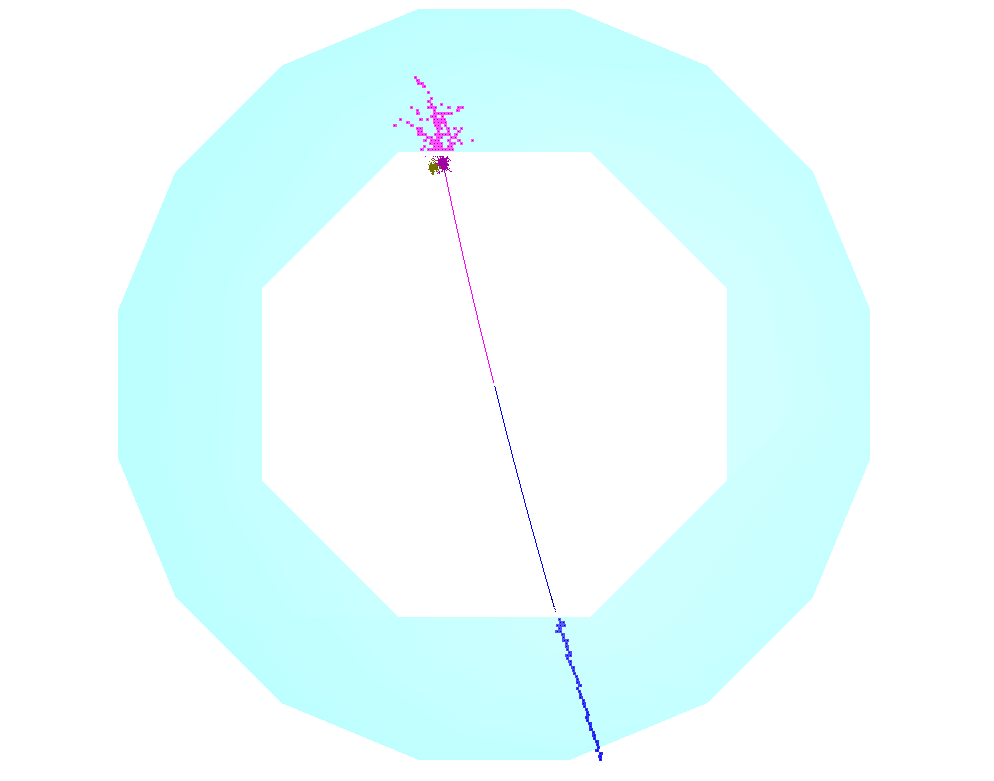
\includegraphics[width=0.5\textwidth]{images/tautauMod}}%

\caption{An event display of a simulated $\Pem\Pep\to \Ptauon\APtauon$ event. The blue region is the cross section of the Electromagnetic Calorimeter barrel region. The top $\Ptau$ decays into a charged $\Ppi$, two photons and neutrinos. The bottom $\Ptau$ decays into a muon and neutrinos.}
\label{fig:Tautau}
\end{figure}

Photon reconstruction is an important part of particle reconstruction. For many physics processes involving particles decaying into photons, such as $\Ptau$ lepton and $\Ppizero$, a good photon reconstruction, which provides a good single photon completeness and purity, as well as a good photon separation resolution, is crucial for reconstructing these particles.

\end{comment}
\section{Overview of photon reconstruction in PandoraPFA}

PandoraPFA provides a framework for particle reconstruction \cite{}, as described in \Section{}. In the linear collider content, it has a vast library of algorithms developed through years by many people. Each algorithm addresses one topological issue in the particle reconstruction \cite{}. The essential part of the PandoraPFA is track-cluster association and reclustering to find the best track-cluster pair. Algorithms that removes trackless clusters, such as removing muon clusters or photon clusters, would provide a clean environment for the track-cluster association, hence improving the jet energy resolution.

Photon identification in the PandoraPFA has two main mechanisms. The basic mechanism tests trackless clusters, the after track-cluster association and the reclustering processes. The second more sophisticated photon identification is performed before the track-cluster association and reclustering process. This algorithm identifies photon electromagnetic shower cores carefully in the dense jet environment.

Second mechanism improves jet energy resolution by correctly identifying photon electromagnetic shower cores and leaving a cleaner environment for the track-cluster association. However, the peripheral calorimeter hits to the shower cores may be left as fragments, and reconstructed as separate particles. This lowers the reconstructed photon completeness and makes the number of reconstructed photons a less useful physical quantity. Also, the second mechanism leaves rooms for improvement of photon separation resolution, illustrated in \Figure{}.

This section presents a solution to the photon fragments issue. The introduced PandoraPFA algorithms also improves the photon separation resolution. Three algorithm will be discussed: a rewritten sophisticated photon reconstruction algorithm, a photon fragment removal algorithm and a photons splitting algorithm.

%The testing simulated data in this paper are generated either by WHIZARD \cite{whizard} or by the simple HepEvt generator. Events are simulated with GEANT4 \cite{Agostinelli:2002hh} in MOKKA \cite{MoradeFreitas:2002kj}. Jet fragmentation was performed with PYTHIA \cite{Sjostrand:1995iq} and the particle reconstruction was done by PandoraPFA \cite{Marshall:2015rfa} in MARLIN reconstruction framework \cite{Gaede:2006pj}, in ILD\_o1\_v6 detector model. The iLCSoft v17-01-07 was used. Different versions of PandoraPFA were used for the comparison purpose.

\section{Overview of photon reconstruction algorithm}

The photon reconstruction algorithm refers to the more sophisticated photon identification of the two main identification mechanism, before the track-cluster association and reclustering process. The algorithm has the following steps: coarsely forming photon clusters, reconstructing photon candidate 

